\documentclass[10pt,a4paper]{report}
\usepackage[utf8]{inputenc}
\usepackage{amsmath}
\usepackage{amsfonts}
\usepackage{amssymb}

%\usepackage{fullpage}
\usepackage{url}
\usepackage[numbers,square]{natbib}
\usepackage{hyperref}
\hypersetup{
	colorlinks,
	citecolor=black,
	filecolor=black,
	linkcolor=black,
	urlcolor=black
}
\usepackage{graphicx}
\usepackage{indentfirst}
\AtBeginDocument{\renewcommand{\bibname}{References}}

\author{Jacek Czyrnek, Adam Koleszar, Marion Le Guével, Mihaly Lengyel}
\title{Group project report}

\begin{document}
\maketitle
\tableofcontents

\chapter{Introduction}
\label{ch:intro}
Optimisation process is a big part in the domain of engineering. It applies for a very wide amount of subjects, and for many, it can be a very heavy and long treatment requiring a lot of resources. That is because of these costs, that a monitoring and recovering system is always needed if any problem could happen during the optimisation process. That way, not all the treatment is lost, and it is not necessary to restart it from the beginning.

This project report is dealing with the purpose of its realization in Chapter \ref{ch:intro}. Then, the previous researches done to define a good recovery system are presented in Chapter \ref{ch:tech}. Chapter \ref{ch:req} explains what the project needs to provide, and Chapter \ref{ch:design} the choices about how to provide it. Finally, Chapter \ref{ch:impl} shows what the project actually looks like, Chapter \ref{ch:test} how the testing phase were handled, and Chapter \ref{ch:fail} what problems were encountered by the team, to end with a conclusion in Chapter \ref{ch:conc}.

\section{Aim and objectives}
The aim of the project itself is to design and develop a distributed system for monitoring the progress of the aerofoil design optimisation through an intuitive user interface with a login access. The main point is not the optimisation, but the recovery system behind it.

As students working in engineering, the objective is to test all the skills needed to do a project. Indeed, it's not only about working in the subject of optimisation or doing an actual monitoring and recovery system, but also working as a team. This means planning and organizing the tasks to design and code the project with a good communication, and to finish with a presentation of what has been done.
	
\section{Distribution of work}
For the documentation of this project, tasks has been split as below:
\begin{itemize}
  \item Adam : Chapter Implementation, Chapter Failure case studies, Chapter Conclusion  
  \item Jacek : Technical review researches, Chapter Implementation, Chapter System testing, Installation and operational manual
  \item Marion : Technical review researches, Chapter Introduction, Chapter Technical review, Chapter Requirement specifications
  \item Mihaly : Technical review researches, Chapter System design
\end{itemize}

\chapter{Technical review}
\label{ch:tech}
All computer systems are composed of many subsystems which can encounter problem or failure preventing them to do their tasks. Because of this, those systems can stop working and, then, loose all their data and progression.

That's why every reliable and secure system takes into account the risk of sudden failure of any of its component. Most of the time, it includes communication between those components and action depending on the analysis of the failure. However, the monitoring and recovery plan is different for each system as each system has its own design and components. Therefore many approaches has been implemented to handle different events of numerous examples of systems. 

\section{Automatic action}
\subsection{Cluster environment}
Cluster systems are complex in a way that it is a distributed environment. This means that there are a lot of independent components communicating together for one common result. Failures can, then, appear on many places. 

A way to locate an error is through a heartbeat protocol \cite{TecReview1,TecReview2} which makes each component send a signal at regular intervals to another one. As soon as the error has been detected, there are different options. 
Some recovery software already exist, but there are very expensive and it requires to install it on every node, paying for each of them \cite{TecReview1}.
You can have a recovery driver which will analyse and execute recovery actions \cite{TecReview1}. If it fails, it will complete the remaining actions anyway. 
There is also a possibility to use a spare server to take over the job. If the heartbeat signal stops, the spare server will do the job instead of the one crashed. However, it means that there is a server inactive most of the time, waiting for a failure, which is a waste of money. This is why Dias \cite{TecReview2} proposes to use a spare server which is actually working with the others even when there is no failure.

\subsection{Software environment}
Software environment can be on a server or on a local machine. It is quite a large form which includes different type of faults. Delgado \cite{TecReview3} exposes the classification of the software fault monitoring system. She explains the use of graphs to detect the violation and call the good function in Java depending of the fault to, finally, enforced the synchronization. To evaluate the error, some measures can be used like tasks performance or other metrics \cite{TecReview4}. A pre-compiler can also be used to correct errors automatically \cite{TecReview5} or a "self-healing" method which reverse faulty until failure is avoided \cite{TecReview6}.
		
\section{User action}	
Many errors can be easily detected during the execution of the system, and, then, automatically handled with pre-determined solutions (see previous section). For other types of errors, it requires the intervention of a human being. 

In a computing environment, a hot key can be selected by the end user at pre-boot or runtime phase to perform a precise recovery action \cite{TecReview7}. This solution is limited by the technical level of the end user as well as the configuration of the computer. 

In a database, once a wrong request has been executed most of the time the only solution is to restore the full database. All the wrong actions are, then, deleted, but also some good ones. Thus, the consistency is lost. Zwilling \cite{TecReview8} suggests to regularly create some snapshots of the change in the database (and not all of it) and some more on specific events. That way, a human being can just go back through some snapshots and find the one that shouldn't be executed without loosing all the other changes.	

\section{Previous researches and current project}
The current project uses an educational Java code from NASA \cite{WWW:NASA} modified to correspond to the current system. This part of the execution is run on a cluster (see Implementation Chapter) but there is no possibility to manage it. That is why handle possible errors can't be done at the infrastructure level. The solution of the logs on the server is the best in this case to track the error and recover from it. 

The main part of the software is on local machine. Therefore, all the results are stored in a local database file. If an error appears in the database, the logs can also restore it.



\chapter{Requirements specifications}
\label{ch:req}
\section{Usecases}
This project handle login as sessions. Therefore each session (a set of iterations) is a new user with a new password.  However, all these "users" are of the same type and have the same functionalities :

\begin{figure}[h!]
	\centering
\includegraphics[width=0.9\textwidth]{Usecase_group-project.png}\\
\caption{Use case}
\end{figure}

Mainly, the purpose of this software is to solve an equation with different given parameters and to display the result graphically.

\section{Functional and non functional requirements}
On the previous use case, different functionalities are written. This subsection will detail those functionalities into functional and non-functional requirements.

\subsection{Functional requirements}
\begin{center}
\begin{tabular}{|c|p{0.8\textwidth}|}
\hline 
\textbf{ID} & \textbf{Requirement} \\ 
\hline 
1 & To log into a session \\ 
\hline 
2 & To create a new session \\ 
\hline 
3 & As logged in : To enter new inputs \\ 
\hline
4 & As logged in : To start or stop iterating on the equation (exchange of data with the cluster) \\ 
\hline
5 & As logged in : To display the result of the iterations in real time on a graph \\ 
\hline
6 & As logged in : To display the result of the iterations in real time as a wing modeling \\ 
\hline
7 & As logged in : To download the log file (exchange of data with the cluster)\\ 
\hline
8 & As logged in : To logout from a session \\ 
\hline
\end{tabular}
\end{center}

\subsection{Non-functional requirements}
\begin{center}
\begin{tabular}{|c|p{0.7\textwidth}|}
\hline 
\textbf{Type} & \textbf{Requirement} \\ 
\hline 
Security & To log into a session with a password so only people having those information can access to it \\ 
\hline 
Reliability & To have a recovery system to access previous steps of a session \\ 
\hline 
Speed & To use a cluster for solving the equation \\ 
\hline
\end{tabular} 
\end{center}

\section{Further information}
An example has been given for the software user interface. With the functionalities required, the final product should have two "pages", one for the connection or creation of a session, and another one once logged in a session, as the mock-ups below:\\
\begin{figure}[h!]
\includegraphics[width=0.9\textwidth]{group_project_mockups.png}
\caption{Mock-up}
\end{figure}

\chapter{System design}
\label{ch:design}
\section{Component diagram}
We began the design process by dividing the system into bigger modules and designing concrete interfaces between them to conduce parallel work. The following diagram shows the components of the system and the interfaces they interact through.

\begin{figure}[h!]
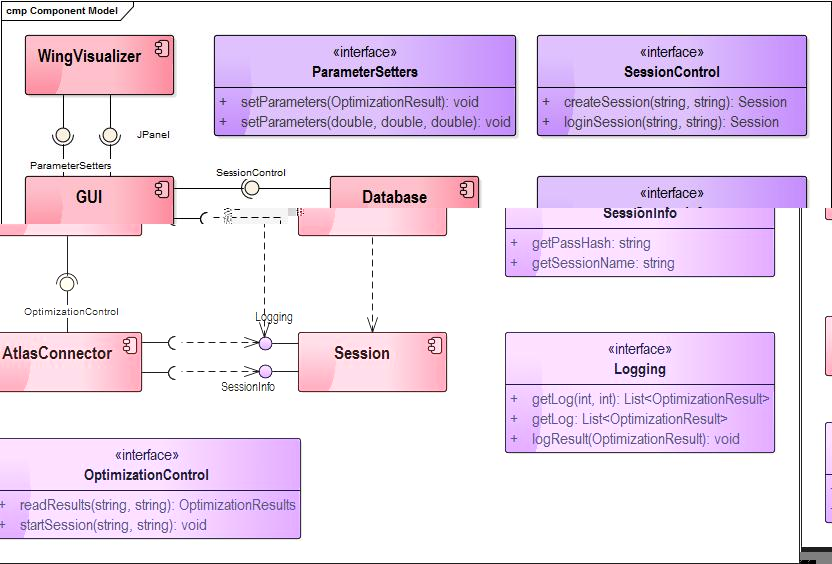
\includegraphics[width=\textwidth]{CompModel.jpg}
\caption{Component diagram}
\end{figure}

We split the software into 4 bigger modules and assigned one to each team member:
 
\subsection{Database \& Session: Marion Le Guével}
These parts of the system are responsible to abstract away the database and session handling. The database module connects the system to a local database and it provides interface to handle the creation and log in of the sessions and logging the results of the optimization. The Session is a simple module, a single class in essence, that is used to pass session information around and to log the results. To make logging possible it depends on the interface provided by the Database module.
\subsection{Astral Connector: Ádám Koleszár}
The AstralConnector module abstracts away the network connection and communication handling. It connects the system to Astral and runs the optimizer on it. It reads the results and logs these in the provided Session. It provides an interface to start and stop an optimization session and requires the logging interface of the Session module to communicate the results of the optimization back to the system. Starting an optimization session is an asynchronous operation, it does everything in a new thread. 

\subsection{Wing Visualizer: Mihály Lengyel}
This module provides means of visualization of the optimization results, namely the shape of the designed wing. It's a subclass of the JPanel class, so it's easily included and displayed in the GUI. It's only provided interface is used to update the currently displayed wing shape.

\subsection{GUI: Jacek Czyrnek}
The GUI connects the rest of the software system together and provides a user interface. It requires interfaces from every other module of the system.
\pagebreak

\section{Class diagram}
In the following diagram you can see, that the classes in the implemented system are simple reflections of the component design above.\\
\begin{figure}[h!]
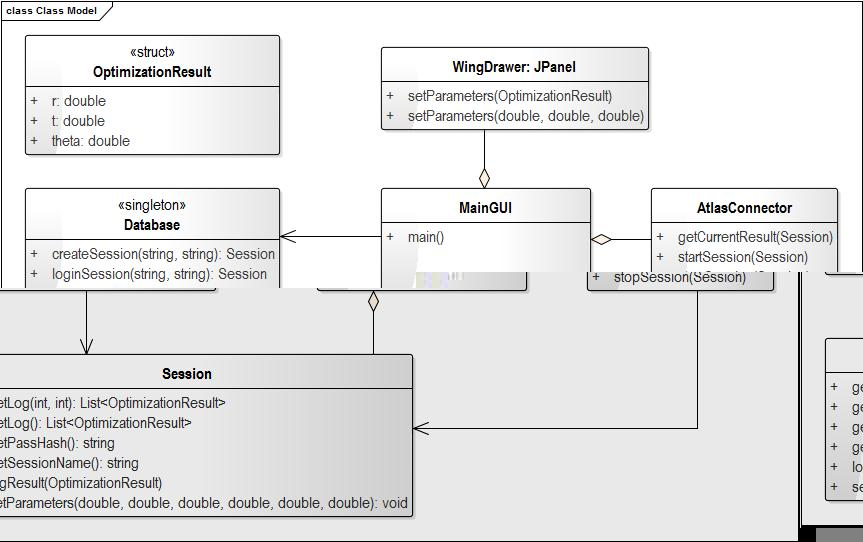
\includegraphics[width=\textwidth]{ClassModel.jpg}
\caption{Class diagram}
\end{figure}
\pagebreak

\section{Sequence diagram}
To complement the static diagrams above here we provide a diagram to show the dynamic behaviour of the system. This is not an exact sequence diagram but it shows the flow of data through the system.\\
\begin{figure}[h!]
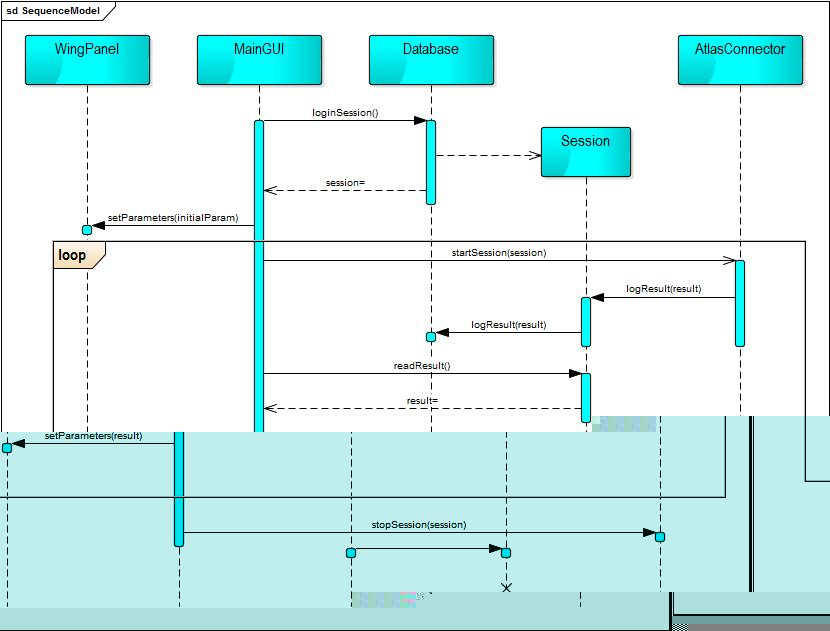
\includegraphics[width=\textwidth]{SequenceModel.jpg}
\caption{Sequence diagram}
\end{figure}\\
\paragraph*{}
As the diagram shows, the main operation of the system starts when the user logs into or creates a session. The previous session data is read from the database and returned as a Session object. The GUI then starts the session using the AstralConnector, which then runs in a different thread. This thread then continuously reads and logs the results using the Session which saves it in the Database. Meanwhile the GUI continues to display and in the display loop it reads the results from the running Session and updates the UI including the WingVisualizer. The GUI stops the running session using through the AstralConnector.

\chapter{Implementation}
\label{ch:impl}
This chapter is about how made the requirements and the design into a working software. For implementation we used JAVA programming language and the Netbeans IDE. For revision control we used github. Our project is accessible at: \url{https://github.com/porcellus/CranfieldUniSETCGroupProject}. We build our code against the Java Development Kit version 1.7. Other libraries used will be mentioned in their relevant sections.

\section{Database}
We used the SQLite single file database solution as our database, and for it to work with our JAVA application we used the open-source SQLite JDBC driver \cite{WWW:SQLite}.

\section{Cluster connection}
As a cluster we used the power of the Astral \footnote{10240 nodes} university cluster, which can be reached via SSH protocol. In order to connect to the servers from our software we used the open-source JSch package from JCraft \cite{WWW:JSCH}. It allowed us the connect to the gate server, copy our solver on it via SCP (secured copy) and start the computation. The result are also coming back on the SSH connection as remote command execution.

For user authentication we created our own handler which uses the interfaces provided by the JSch package. It handles the password prompt and other connection configuration as well silently, so the user only need to type in his or her user name and password.

\subsection{Remote computation}
Although our software contains the solver component as well, due Java version differences on the Astral server we decided to create a separate software that handles the computation and can run on the remote machines.

It is a command line application. It has several parameter options. To handle these command line parameters we used the open-source CLI commons package from Apache \cite{WWW:CLI}.

\subsubsection{Solver}
It is based on the previously mentioned NASA air foil simulation educational JAVA applet \cite{WWW:NASA}. Because it contained computation for several other environment that is different for the normal Earth conditions we removed most irrelevant parts from it. The solver now can compute dimensionless lift and drag forces for given wing geometrics.

\subsubsection{Optimizer}
The optimizer is also part of the remote program. It takes parameter intervals for the wing geometrics and optimizes the lift drag ratio between those intervals returning the optimized wing geometrics. It also logs whenever a better solution is found.

\section{Wing visualiser}
The panel that displays the image of the wing and the surrounding air flow is based also on the NASA applet \cite{WWW:NASA}. We extracted the minimal amount of code from that project to display the wing properly. It is then included in the main GUI frame as a panel.

\section{GUI}
All mentioned modules work behind the graphical user interface build from the components of Swing widget toolkit. It consists of the main frame controlling visibility and interacting in between login/session creation dialog, parameters input dialog and session panel. The JFreeChart library \cite{WWW:JFreeChart} has been used to generate chart representing the lift-to-drag ratio.

\chapter{System testing}
\label{ch:test}
\section{Unit testing}
For unit testing we used the most obvious choice regarding JAVA software, the JUnit package. It is included in several JAVA enabled IDE (Eclipse, Netbeans). It enabled us to test most classes of the system. Luckily most of our modules connected through interfaces so when testing a particular class that uses other classes from other packages, we just implemented a small stub version of the external classes. With them we could concentrate the testing to our actual unit.

\section{User interface testing}
As most of the user interface elements requires actual user input we omitted unit testing of these part as they cannot be automated with our current tool set.  Instead we used manual testing of these components. We tested the input fields for malformed, corrupted and missing inputs. Tested every dialog for cancellation as well.

\section{Validating the solver}
As the solver component came from external source we assumed that proper testing was done on their so we only validated our stripped down version of the solver against the full applet manually. We gave the same parameters to the applet and to our solver and compared the results.

\section{Database testing}
Because the SQLite database does not have any server-like interface, only an API, we checked the results of our database calls with an external tool: SQLiteBrowser \cite{WWW:SQLiteBr}. With this tool we could see inside every table and every record of the created database to check if our calls are working.

\chapter{Failure case studies}
\label{ch:fail}
In this chapter we are going to write about the various failures that can occur during execution of the program and the way they can be avoided or repaired.

\section{Communication errors}
For a system that uses external connections to transfer data between components (like a network) is bound to have some communication errors in time. These can be disconnection issues, data corruption, security issues. As programmers we have to ensure that the system will properly handle these issues without too much data loss.

Failure to do so will lead to the waste of significant computation effort, which can be ultimately translated to the loss of money and time. To avoid or to be prepared for these cases the following measures were taken.

\subsection{Disconnection}
If a network connection disconnects it is only allowed to lose the data being sent, nothing more. For this, proper and thorough logging system needs to be implemented. In our case it is client and server side logging as well.

\subsection{Server side logging}
On the server side simple log files are created. Every line contains the best solution at that point in time. The solution contains the angle of attack, the camber size relative to the chord and the thickness of the wing relative to the chord. The solution also contains the computed the dimensionless values of the lift and drag forces and the ratio of the two for easier data readability. The help the finding of data on the server the log files are named after the session name.

\subsection{Client side logging}
The sessions and the computed values are also logged on the client side of the application. These data are stored in the SQLite database file attached to the program. From that any computation session and it's result can be restored and even continued if the computation didn't finish.

\subsection{Transfer error}
If the messages between the server and the client side get corrupted for any kind of reason, the messages will get discarded, and user will get a notification about possible communication error. The computation will continue and produce relevant data on the server side. If the data in between is not relevant the results can be gathered from the server log, if they are relevant as well, the computation can continue from the last correct message.

\subsection{SSH related errors}
Before the computation could start the program needs to copy the computing part of the program to the remote machine. During these communications errors can occur either with the connection itself, or with the SSH protocol. Later errors include SSH server downtime, user authentication errors etc. Dealing with these issues is outside of the scope of our program, although the program will do anything so that no data should get lost. The program will notify the users about SSH errors, and computation won't start until such issues are handled.

\section{Database error}
Database error can rearrange from small communication problems with the server to large crashes that can destroy the whole database. In our case the SQLite solution is a one-file database, so it does not rely on any kind of network communication. So most of the errors that can happen to our database are file related errors. File deletion, file corruption, disk errors etc. could lead to the complete loss of our database. That is why it is important to regularly back-up this file and restore it to a previous save when needed.

\section{Software error}
Software errors include problems that can be originated from the implementation of our software. Despite all testing efforts a program can still break for various reasons that need to be addressed in order to avoid or minimize data loss. 

\subsection{Server side error}
Bad input parameters can lead to undefined behaviour, that is why parameter checks should be carried out before execution. It is only done on the client side, so the server side part is not designed to work independently (although nothing prevents to user to actually run it without the client side).

The program also uses a computational method so we should take into consideration the numerical behaviour of the algorithm. The method we are using is not that complicated and can converge relatively easily, so we don't expect numerical errors.

\subsection{Client side error}
Typical parameter errors on the client side includes bad user name or password, for which the program will ask a re-entry. If the user wants to create a previously existing session the program won't let it, and warns the user to either load the existing session or create a new one.

Parameters for the optimizer are limited by spinners. Failing to change one parameter will always set its value to the default which will run without problems. The wing visualiser will draw the wing according to the received data. If the connection is failing the visualiser will draw the last received results.


\chapter{Conclusion}
\label{ch:conc}
This chapter concludes the work we have done on this project. By the deadline we were able to present a working program that is able to compute geometrics for an air foil with optimal lift drag ratio with the help of a cluster. It is also able to log its results recover from them if any error occurs during runtime or otherwise. 

We were also able to present its features and properties, and demonstrate a working version of the program, during the presentation. 

This group project was a good exercise to make us use all the knowledge we gathered throughout the last semester, and provided a quick introduction into making a complete product through teamwork.

Here is a quick list to demonstrate which lectures were relevant in the making of this project.
\begin{itemize}
	\item JAVA programming
	\item High performance computing
	\item Requirements analysis and system design
	\item Software testing and quality assurance
	\item Management (teamwork, organising, presentation)
\end{itemize}

\begin{flushleft}
	\bibliographystyle{plain}
	\bibliography{bibliography}
	\addcontentsline{toc}{chapter}{References}
\end{flushleft}

\end{document}
